%\documentclass[12pt,a4paper]{article}
%\usepackage[ngerman]{babel}

\documentclass[12pt,a4paper,final]{article}
\usepackage[T1]{fontenc}
\usepackage[utf8]{inputenc}
\usepackage[ngerman]{babel}
\usepackage{amsmath}
\usepackage{amsfonts}
\usepackage{amssymb}
\usepackage{lmodern}
\usepackage[left=2cm,right=2cm,top=2cm,bottom=2cm]{geometry}
\usepackage{graphicx}
\title{BCDWristWatch}
\date{\vspace{-10ex}}
\begin{document}
\pagenumbering{gobble}
\maketitle
\section{PCB}

\subsection{First PCB Version}
The First PCB Version was a desaster. The PCBs arrived very fast, but the QFN Package had the wrong size.
ATMEL only produces QFN32 in 7x7mm. Therefore the design of the PCB hat to be changed to the smaller package,
but that gave me the Chance to shrink the Design to a smaller form factor.
The part which keeps the PCB from getting smaller is the Coin Cell Battery (CR2032).
On the PCBs there was the order number printed on the Front side, which would be visble in the final assembly.
\subsection{Second PCB Version}

The second PCB Version was designed from scratch. But the Front was the side with the Battery, so hopefully the Order Number would not be printed on the visible side of the PCB. This worked out very well for the second Version of the PCBs.
\subsection{PCB1}

since the PCBs finally arrived. it was possible to assemble all the parts.
The first PCB was assembled with some Cables soldered to the Testpins on the Backside of the Board.
And the Battery case was also not assembled.
Here is a Picture of the uncleaned but already soldered PCB
\begin{figure}
\begin{center}
  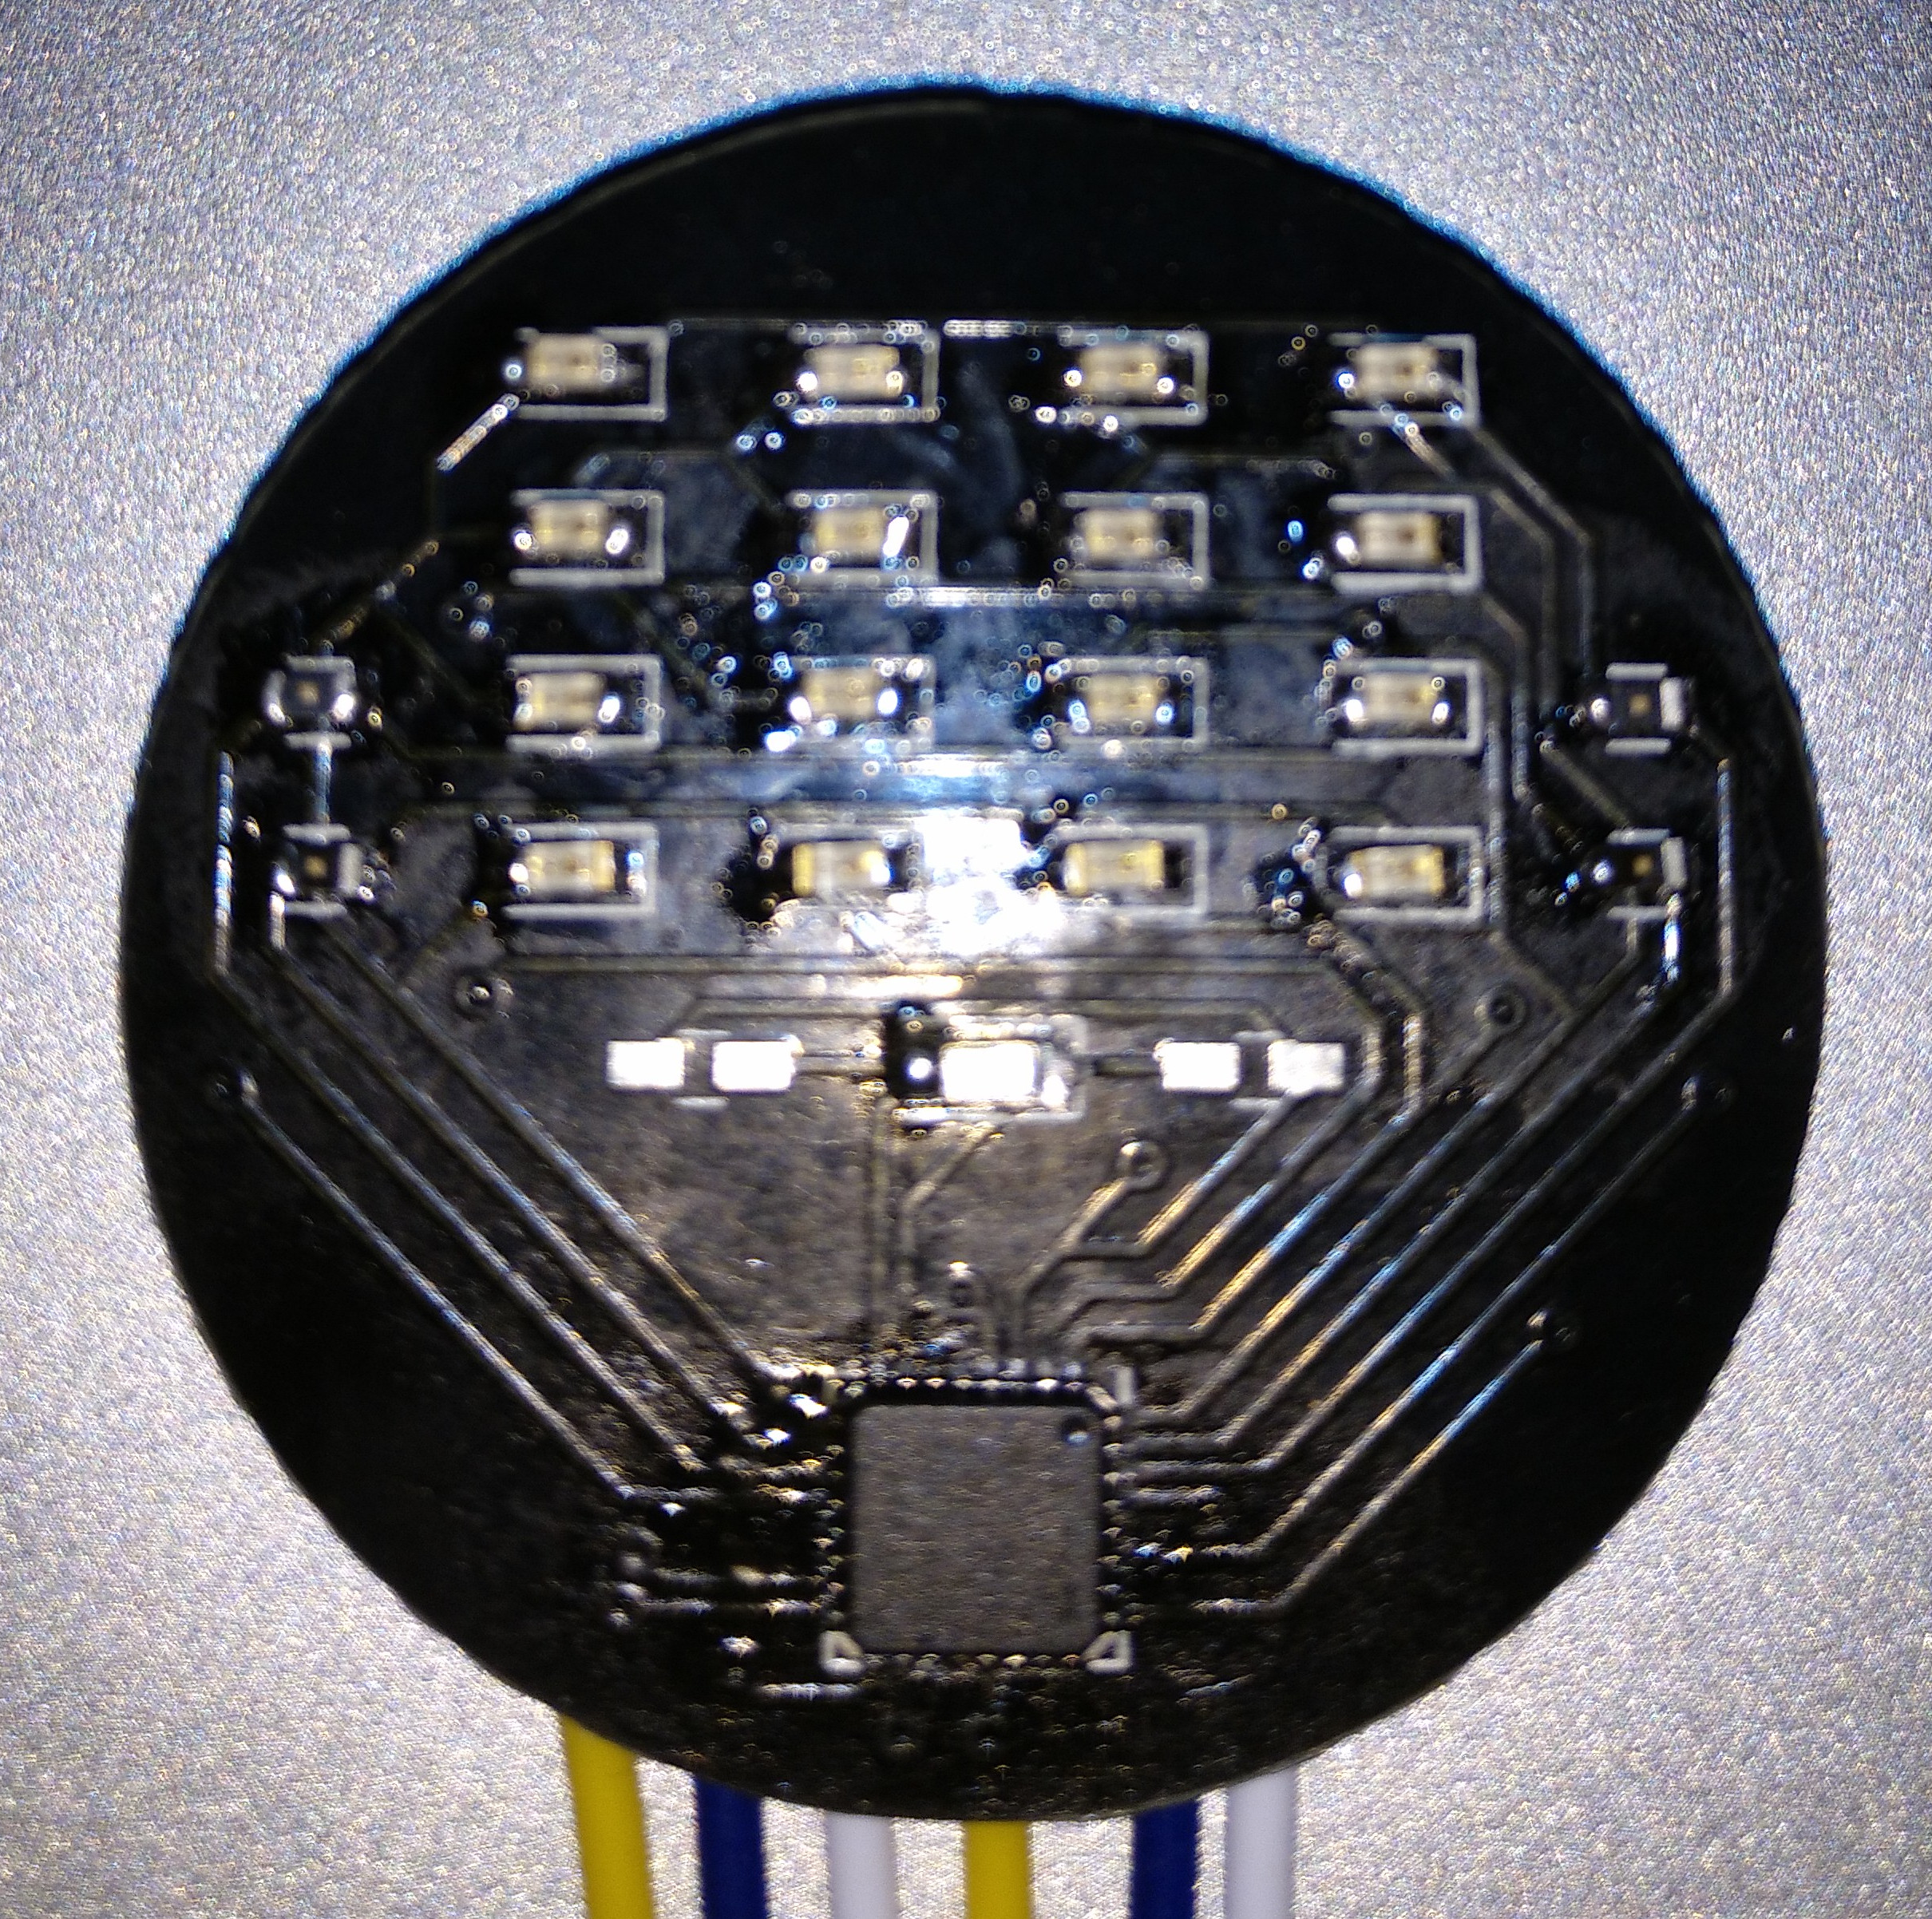
\includegraphics[width=0.5\textwidth]{../Pictures/PCB1_F1.jpg}
  \caption{first PCB}
\end{center}
\end{figure}
\end{document}
